\documentclass[11pt,a4paper]{article}
\usepackage{url,hyperref,lineno,microtype,subcaption}
\usepackage{color,tensor,multirow,siunitx}
\usepackage[onehalfspacing]{setspace}
\usepackage{makecell}
\renewcommand{\cellalign}{cl}
\renewcommand{\rmdefault}{phv}
\usepackage{amsmath}
\usepackage{amsfonts}
\usepackage{amssymb}
\usepackage{graphicx}
\usepackage[round]{natbib}
\usepackage{apalike}

\setlength{\parindent}{0pt}
\setlength{\parskip}{5pt}

\usepackage{caption}
\captionsetup[figure]{name=Fig., labelfont=bf}

\renewcommand{\cellalign}{cl}

\newcommand{\ds}{\displaystyle}
\newcommand{\nl}{\ \\ }
\newcommand{\ud}{\textrm{ d}}
\newcommand{\bs}{\bigskip}

\newcommand{\bu}{\mathbf{u}}
\newcommand{\bv}{\mathbf{v}}
\newcommand{\bx}{\mathbf{x}}
\newcommand{\be}{\mathbf{e}}
\newcommand{\bb}{\mathbf{b}}
\newcommand{\bk}{\mathbf{k}}
\newcommand{\bn}{\mathbf{n}}
\newcommand{\bR}{\mathbf{R}}

\definecolor{red}{rgb}{1,0,0}
\definecolor{blue}{rgb}{0,0,0.8}
\definecolor{green}{rgb}{0,0.5,0}
\newcommand{\emphc}[1]{\emph{\textcolor{red}{#1}}}
\newcommand{\modif}[1]{\textcolor{red}{#1}}
\newcommand{\hycom}{\textsc{hycom} }
\newcommand{\slim}{\textsc{slim}\ }
\newcommand{\ie}{{\it i.e.}\ }
\newcommand{\eg}{{\it e.g.}\ }
\newcommand{\edit}[1]{\textcolor{orange}{#1}}
\newcommand{\UV}{\mathbf{U}}
\linenumbers


\title{Development of a coupled current-wave model to assess the impact of a hurricane on particle transport}
\author{Thomas Dobbelaere, Emmanuel Hanert}

\begin{document}

\maketitle
\begin{abstract}
In most hydrodynamic model studies, currents and waves are simulated separately. This is especially true for the simulation of passive drifters, whose trajectories are often computed based solely on currents. Although this simplification holds for most situations, as the force exerted by waves on currents can be neglected in fair weather conditions, it may lead to significant errors in storm conditions, during which local currents are strongly influenced by wind-generated waves. In this study,current-wave interactions in heavy-wind conditions  are studied by coupling the unstructured-mesh hydrodynamic model SLIM with the wave model SWAN in the Florida Reef Tract during Hurricane Irma (Sep. 2017). This coupled model successfully reproduced both the observed wave behavior and storm surge during the hurricane. The modeled currents were then used to simulate the trajectories of passive drifters during the passage of the hurricane. Our results show that taking wave force into account induces  variations of up 1 m/s in modelled currents on the continental shelf break as well as in the vicinity of  reefs and islands. Wave-current interactions can therefore strongly modify  the transport of drifting material, such as sediments and coral larvae, during heavy-wind events. That should in particular affect connectivity modeling studies since coral mass spawning events tend to occur during the hurricane season in the Caribbean.

\end{abstract}

% === INTRODUCTION === %
\section{Introduction}


% === METHODS === %
\section{Methods}
\subsection{Wind and atmospheric pressure for Hurricane Irma}
\begin{itemize}
    \item Reduction of wind speed according to \cite{harper2010guidelines}
    \item HURDAT 2 \citep{landsea2013atlantic} for hurricance pressure with radius of maximum wind speed according to \cite{knaff2018statistical} using Holland pressure profile \citep{lin2012hurricane}.
\end{itemize}
\subsection{Hydrodynamic model}
Ocean currents generated during hurricane Irma in the Florida Reef Tract (FRT) were modelled using the unstructured-mesh depth-integrated coast ocean model SLIM\footnote{\url{https://www.slim-ocean.be}}. The model mesh covers an area similar to the model extent of \cite{dobbelaere2020coupled}, that includes the FRT but also the Florida Strait and part of the Gulf of Mexico (Figure \ref{fig:mesh}). However, this area has been slightly extended northeastward and westward in order to include the location of buoys for wave outputs validation. Furthermore, in order to withstand potential cell drying due to storm conditions in this study, we used the conservative mode of SLIM with wetting-drying, whose equations write:
\begin{equation}
    \begin{split}
        \dfrac{\partial H}{\partial t} +\nabla\cdot(\UV) =& ~0 \\
        \dfrac{\partial \UV}{\partial t}  + \nabla\cdot\left(\dfrac{\UV\UV}{H}\right) =& -f\mathbf{e}_z \times \UV + \alpha gH\nabla(H-h) - \dfrac{1}{\rho}\nabla p_\text{atm} + \dfrac{1}{\rho}\text{\boldmath$\tau$}_s \\
         &+\nabla\cdot(\nu\nabla\UV) - \dfrac{C_b}{H^2}|\UV|\UV + \gamma(\UV_\ast-\UV)
    \end{split}
\end{equation}
where $H$ is the water column height and $\UV$ is the depth-averaged transport; $f$ is the Coriolis coefficient; $g$ is the gravitational acceleration; $h$ is the bathymetry; $\alpha$ is a coefficient stating whether the mesh element is wet ($\alpha=1$) or dry ($\alpha=0$); $\nu$  is the viscosity; $C_b$ is the bottom drag coefficient; $\nabla p_\text{atm}$ is the atmospheric pressure gradient; {\boldmath$\tau$}$_s$ is the surface stress due to wind; and $\gamma$ is a relaxation coefficient towards a reference transport $\UV_\ast$. As in \cite{frys2020fine} and \cite{dobbelaere2020coupled}, SLIM currents were relaxed towards HYCOM \citep{chassignet2007hycom} in regions where the water depth exceeds a given threshold. At very high wind speeds, the white cap is blown off the crest of the waves, which generates a layer of droplets that acts as a slip layer for the winds at the ocean-atmosphere interface \citep{holthuijsen2012wind}. This causes a saturation of the wind drag coefficient for strong winds \citep{donelan2004limiting,powell2003reduced}. To account for the impact of this saturation on the surface wind stress in our model, we implemented the wind drag parameterization of \cite{moon2007physics}.

The mesh resolution depended only on the distance to coastlines and reefs, bathymetry and bathymetry gradient in order to satisfy SWAN refinement criterion $h/A\geq a$, where $h$ is the water depth and $A$ is the element area. The mesh was generated using the Python library seamsh\footnote{\url{https://pypi.org/project/seamsh/}}, based on the the open-source mesh generator GMSH \citep{geuzaine2009gmsh} and is composed of approximately 7.7 $\times$ 10$^5$ elements. The coarsest elements, far away from the FRT, had a characteristic length size of about 5 km. Figure \ref{fig:mesh} depicts how a 100-m spatial resolution mesh simulated fine-scale details of the ocean currents and significant wave height generated by hurricane Irma in the Florida Keys.

\begin{figure}
    \centering
    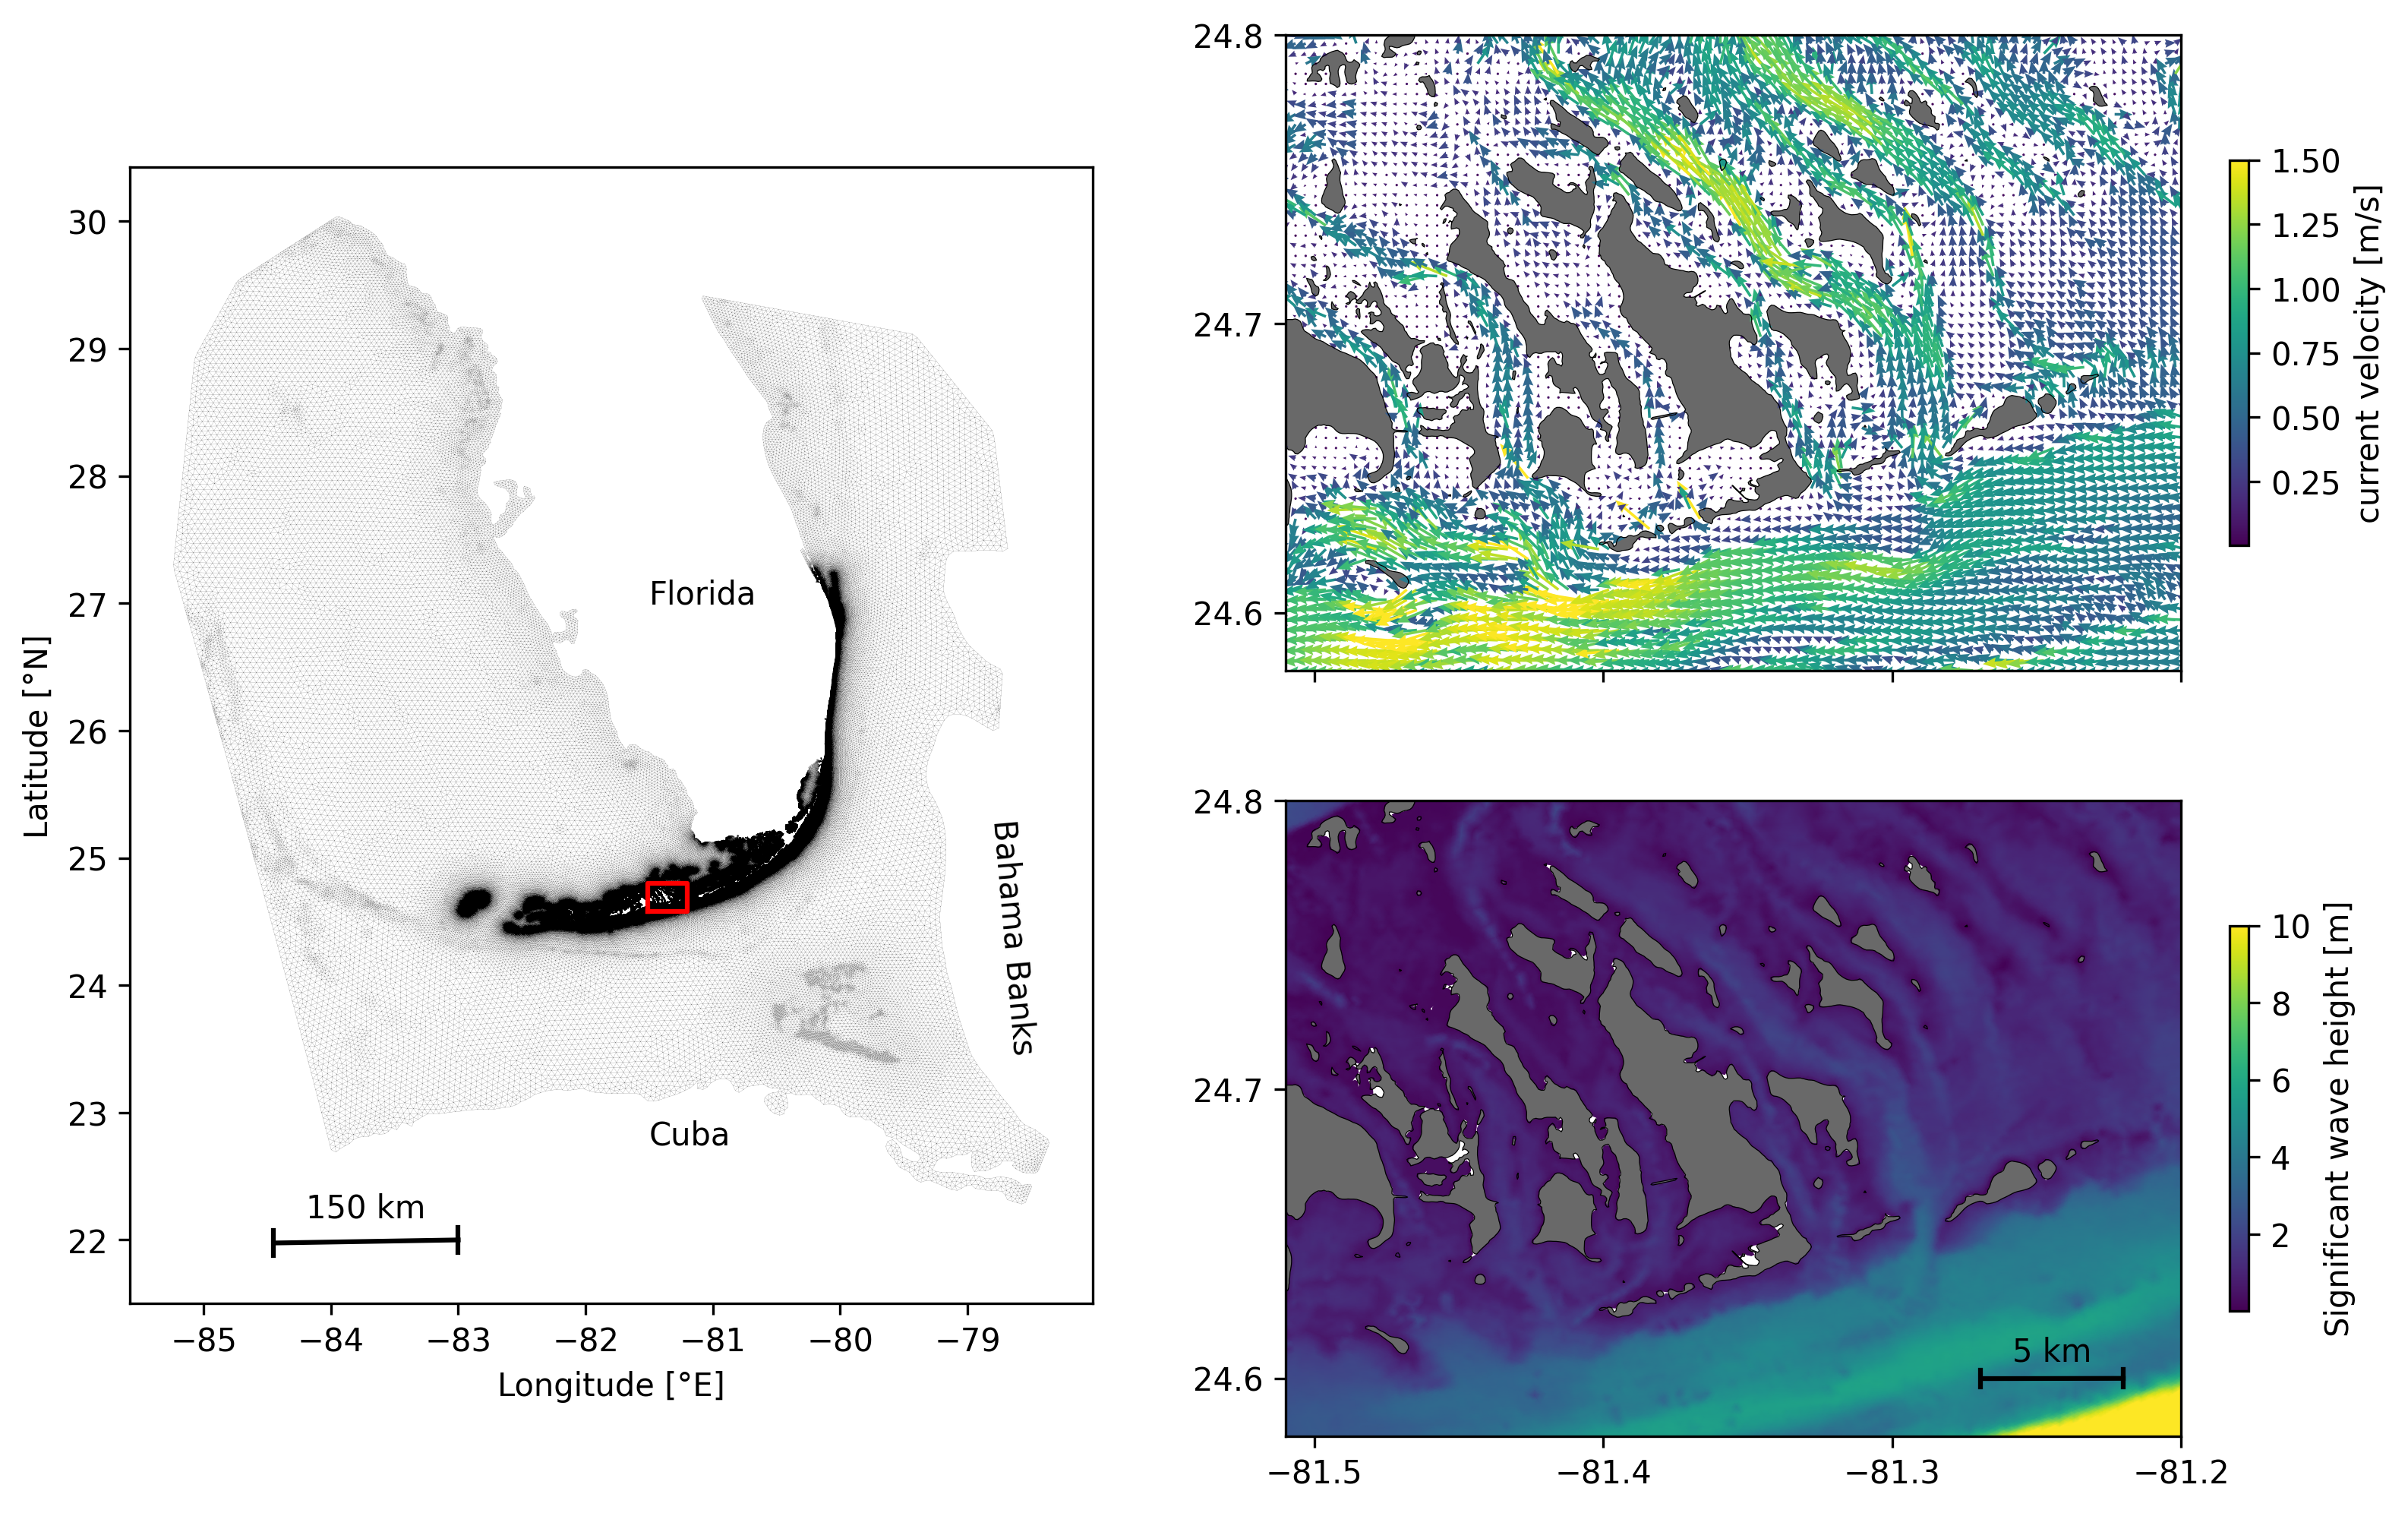
\includegraphics[width=.95\textwidth]{fig/fig_mesh_ww3.png}
    \caption{Mesh of the computational domain with snapshots of simulated instantaneous currents and significant wave height on 2017-09-10 at 11:00:00. The mesh resolution ranges from 100 m in the Florida Keys to a maximum of 5 km offshore.}
    \label{fig:mesh}
\end{figure}
\subsection{Wave model}
Waves were modelled using parallel unstructured SWAN \citep{booij1999third} on the same mesh as SLIM. This model solves the action balance equation, which reads \citep{mei1989applied}:
\begin{equation}
    \dfrac{\partial N}{\partial t} + \nabla_\mathbf{x}\cdot[(\mathbf{c}_g+\mathbf{u})N] + \dfrac{\partial }{\partial \theta}[c_\theta N] + \dfrac{\partial}{\partial \sigma}[c_\sigma N] = \dfrac{S_{in}+S_{ds}+S_{nl}}{\sigma}
\end{equation}
where $N$ is the wave action density; $\theta$ is the wave propagation direction; $\sigma$ is the wave relative frequency; $\mathbf{c}_g$ is the wave group velocity, $\mathbf{u}$ is SLIM depth-averaged current velocity; $c_\theta$ and $c_\sigma$ are the propagation velocities in spectral space due to refraction and shifting in frequency due to variations in depth and currents; and $S_{in}$, $S_{ds}$, and $S_{ds}$ respectively represent wave growth by wind, wave decay and nonlinear transfers of wave energy through interactions between triplets and quadruplets. Spectra were discretized with 48 direction bins and 50 frequency bins logarithmically distributed from 0.3 to 2 Hz. Exponential wind growth was parameterized using the formulation of \cite{janssen1991quasi}, while dissipations by whitecapping and bottom dissipations followed the formulations of \cite{komen1984existence} and \cite{madsen1989spectral} respectively. Coefficients for exponential wind growth and whitecapping parameterizations were based on the results of \cite{siadatmousavi2011evaluation}. Finally, wave boundary conditions were derived from WAVEWATCH III \citep{tolman2009user} spectral outputs at buoy locations.
\subsection{Coupled model}
Express $z_0$ for Madsen bottom friction from Manning dissipation used in SLIM obtained following the methodology of \cite{dietrich2011hurricane}

%%%%%%%%%%%%%%%%%%%
% --- RESULTS --- %
%%%%%%%%%%%%%%%%%%%
\section{Results}

\subsection{Validation}
\begin{figure}
    \centering
    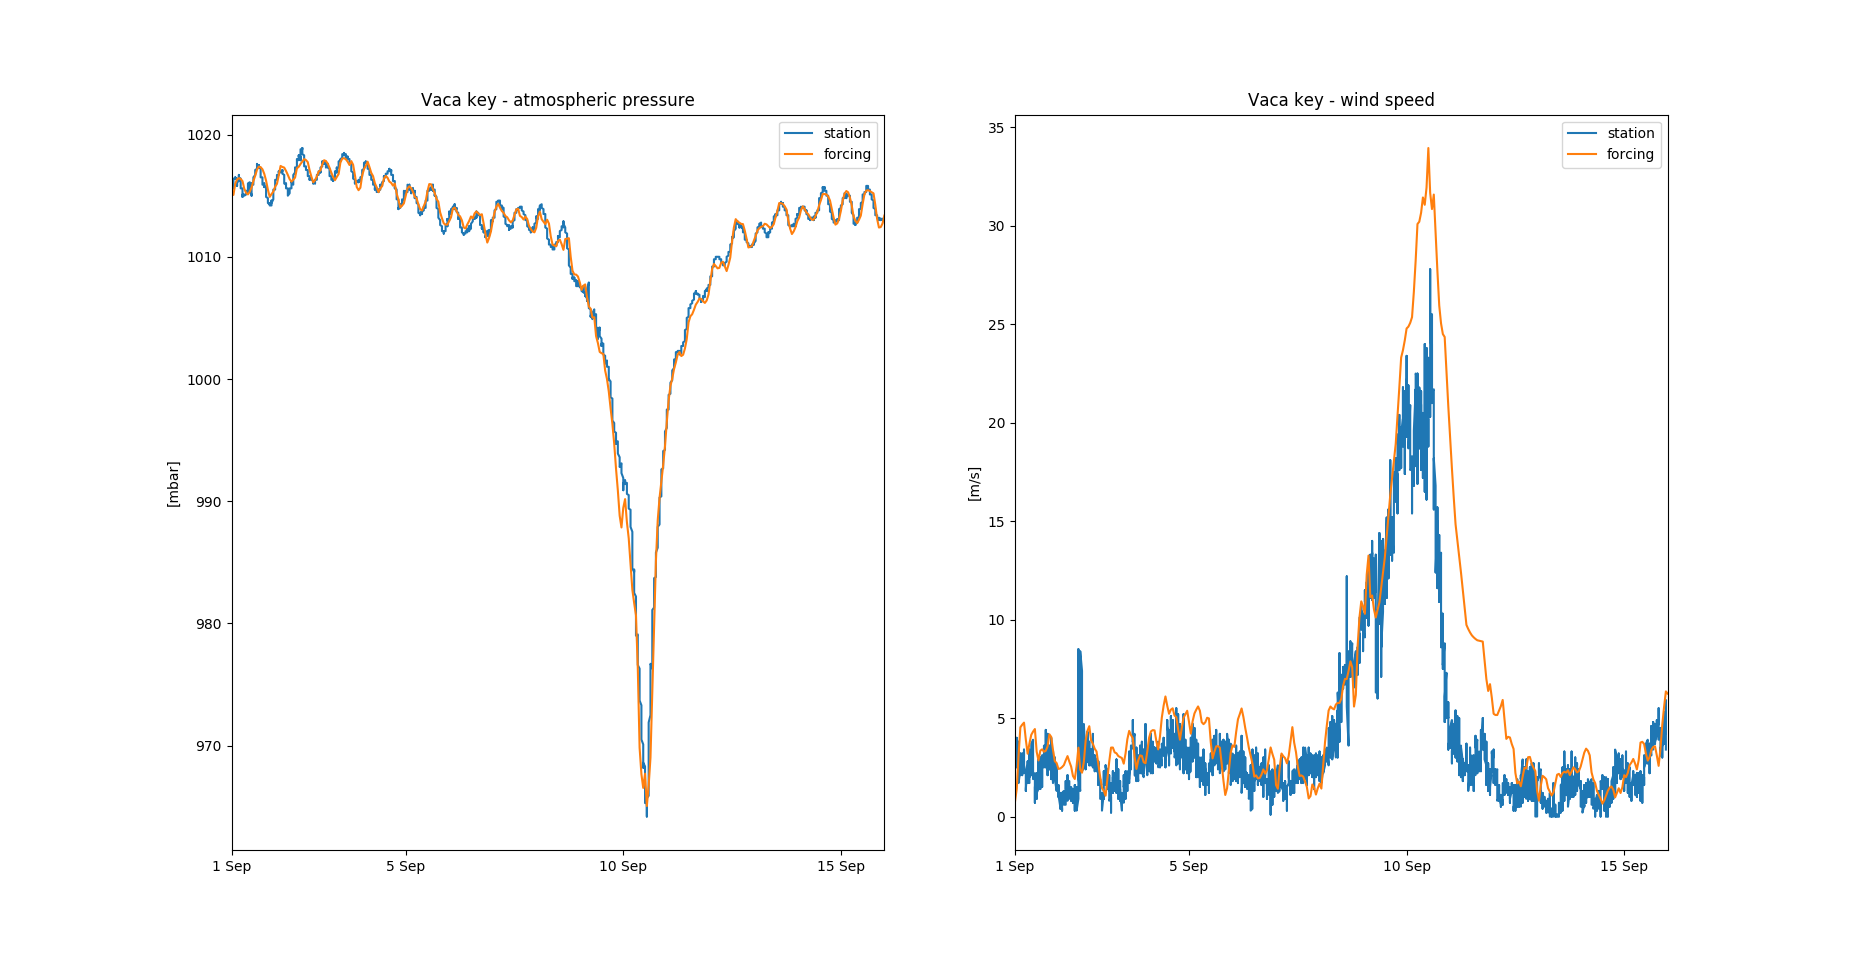
\includegraphics[width=.95\textwidth]{fig/validation_met.png}
    \caption{The atmospheric forcings have been validated with meteorological station observations at Vaca Key. The reconstructed atmospheric pressure and wind speed agree well with field measurements.}
    \label{fig:forcings}
\end{figure}

\begin{figure}
    \centering
    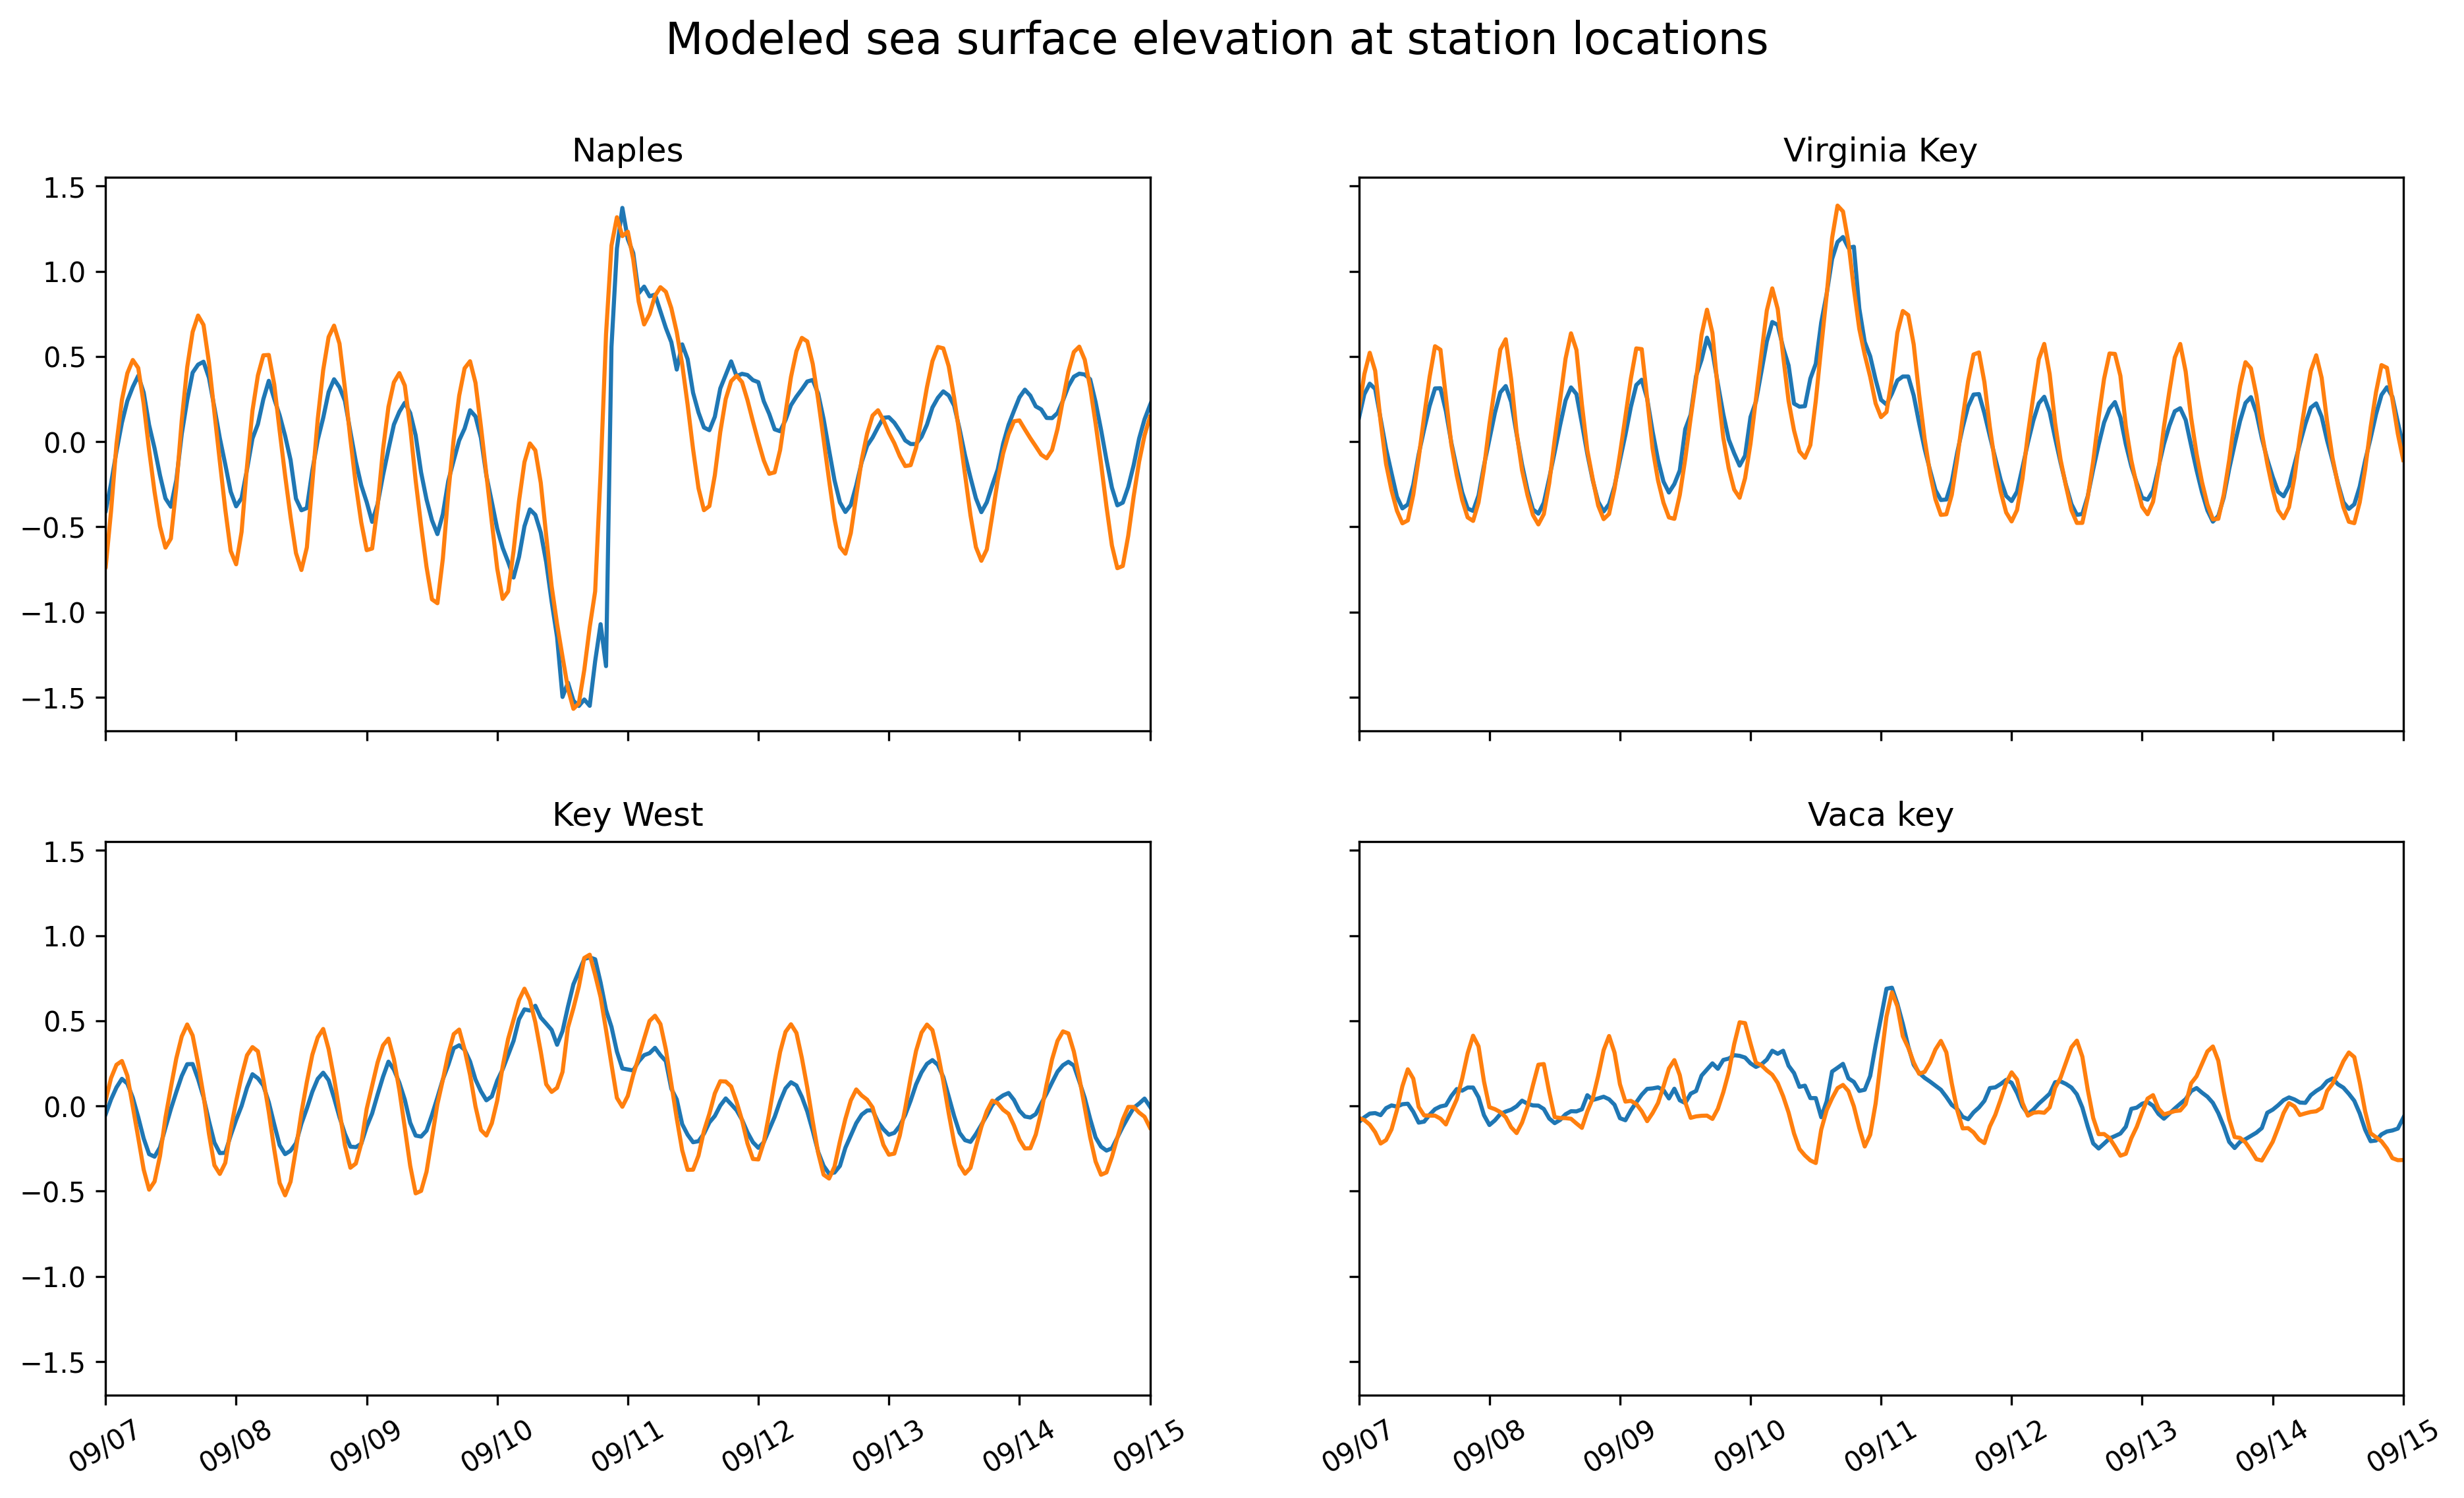
\includegraphics[width=.95\textwidth]{fig/elevation_with_map.png}
    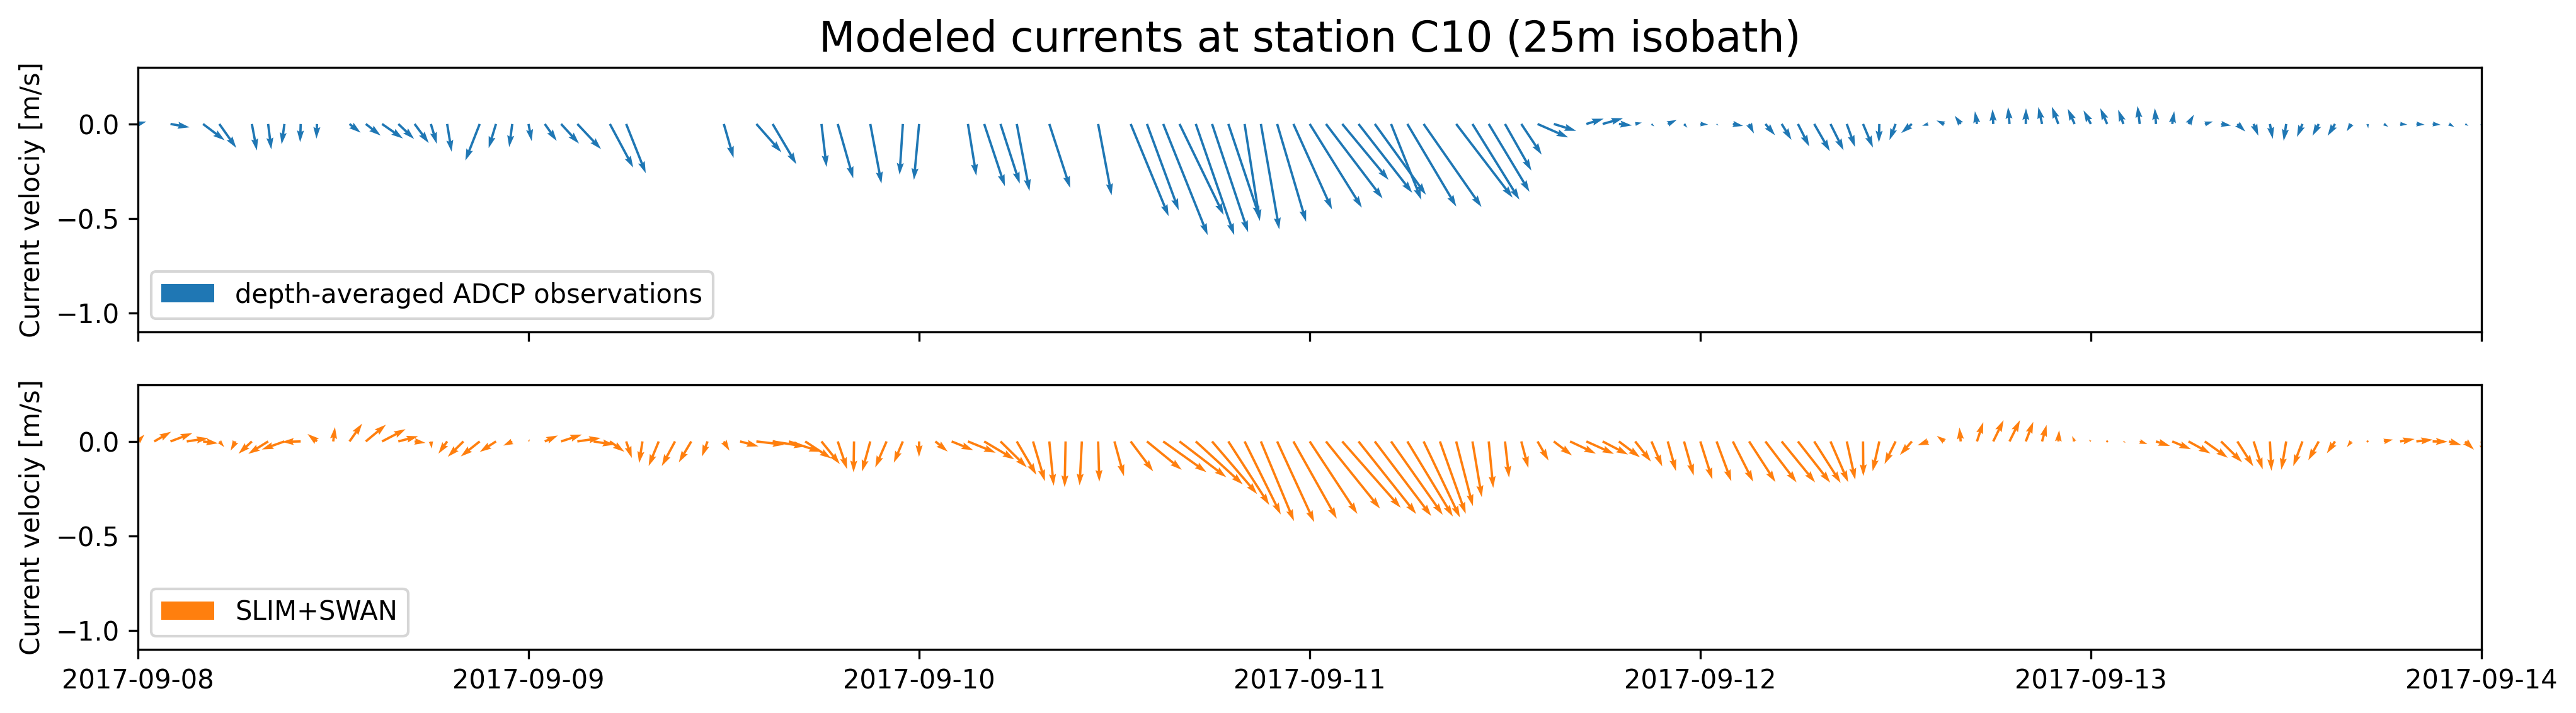
\includegraphics[width=.95\textwidth]{fig/validation_currents_C10_ww3.png}
    \caption{The sea-surface elevation produced by the coupled wave-current model agrees with SSE and current velocity observations at different stations. The fit is particularly good in the Florida Keys and in Naples, on the inner Florida shelf. The coupled model currents have been validated against current meter data on the inner Florida shelf. The current speed and direction during the hurricane agrees well with the observations.}
    \label{fig:hydro}
\end{figure}

\begin{figure}
    \centering
    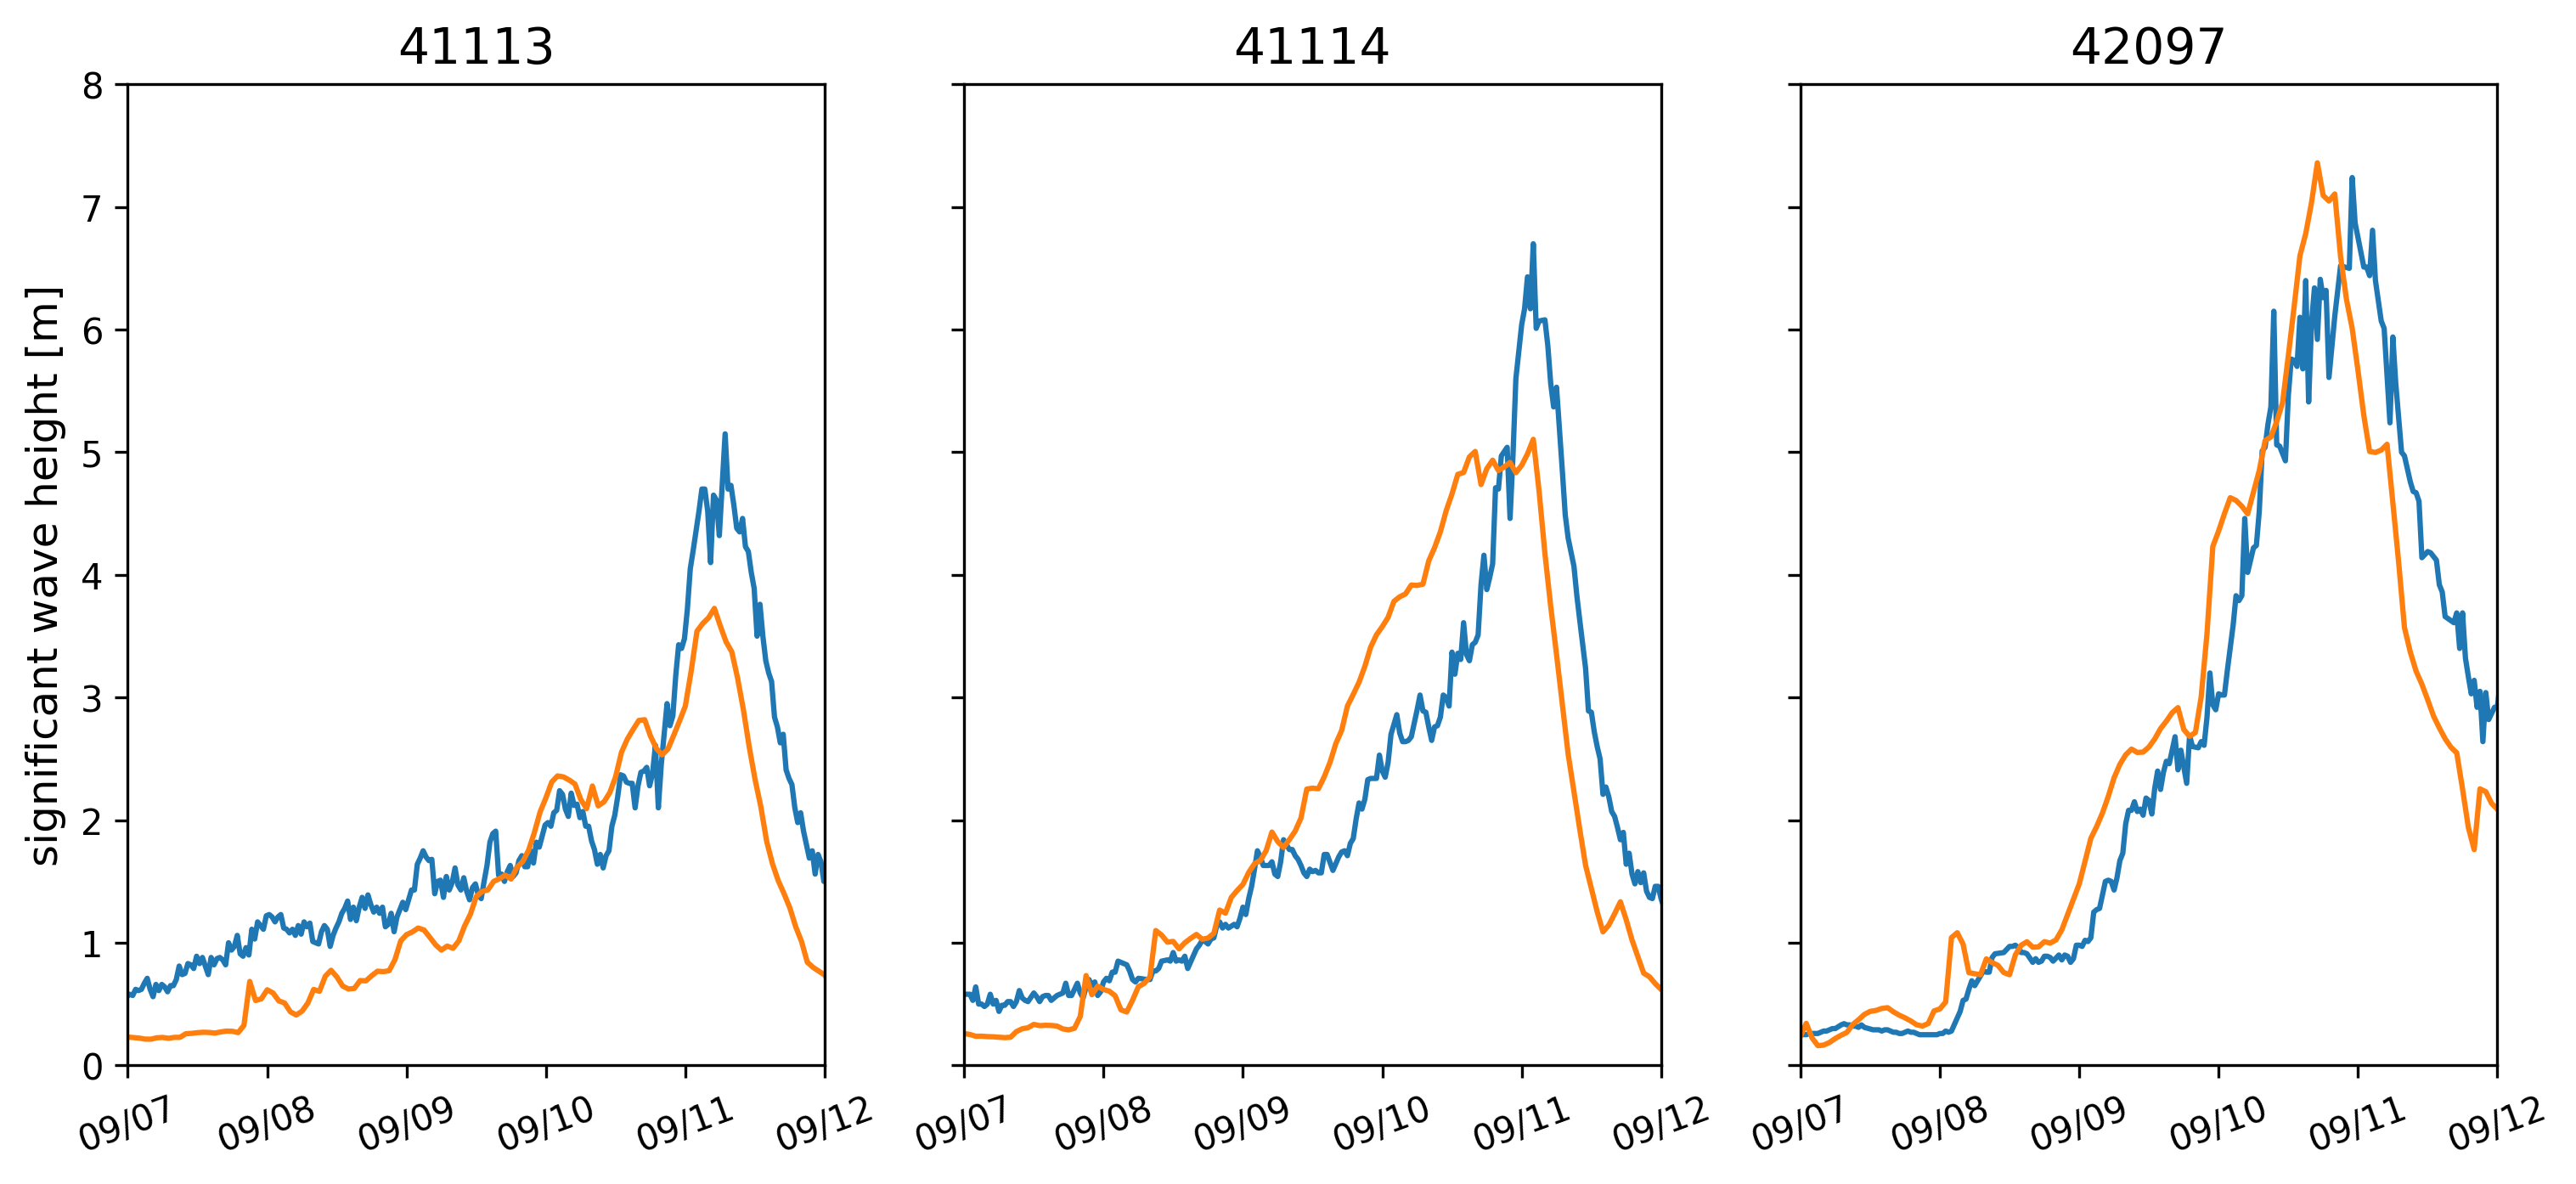
\includegraphics[width=.95\textwidth]{fig/hsig_with_map_ww3.png}
    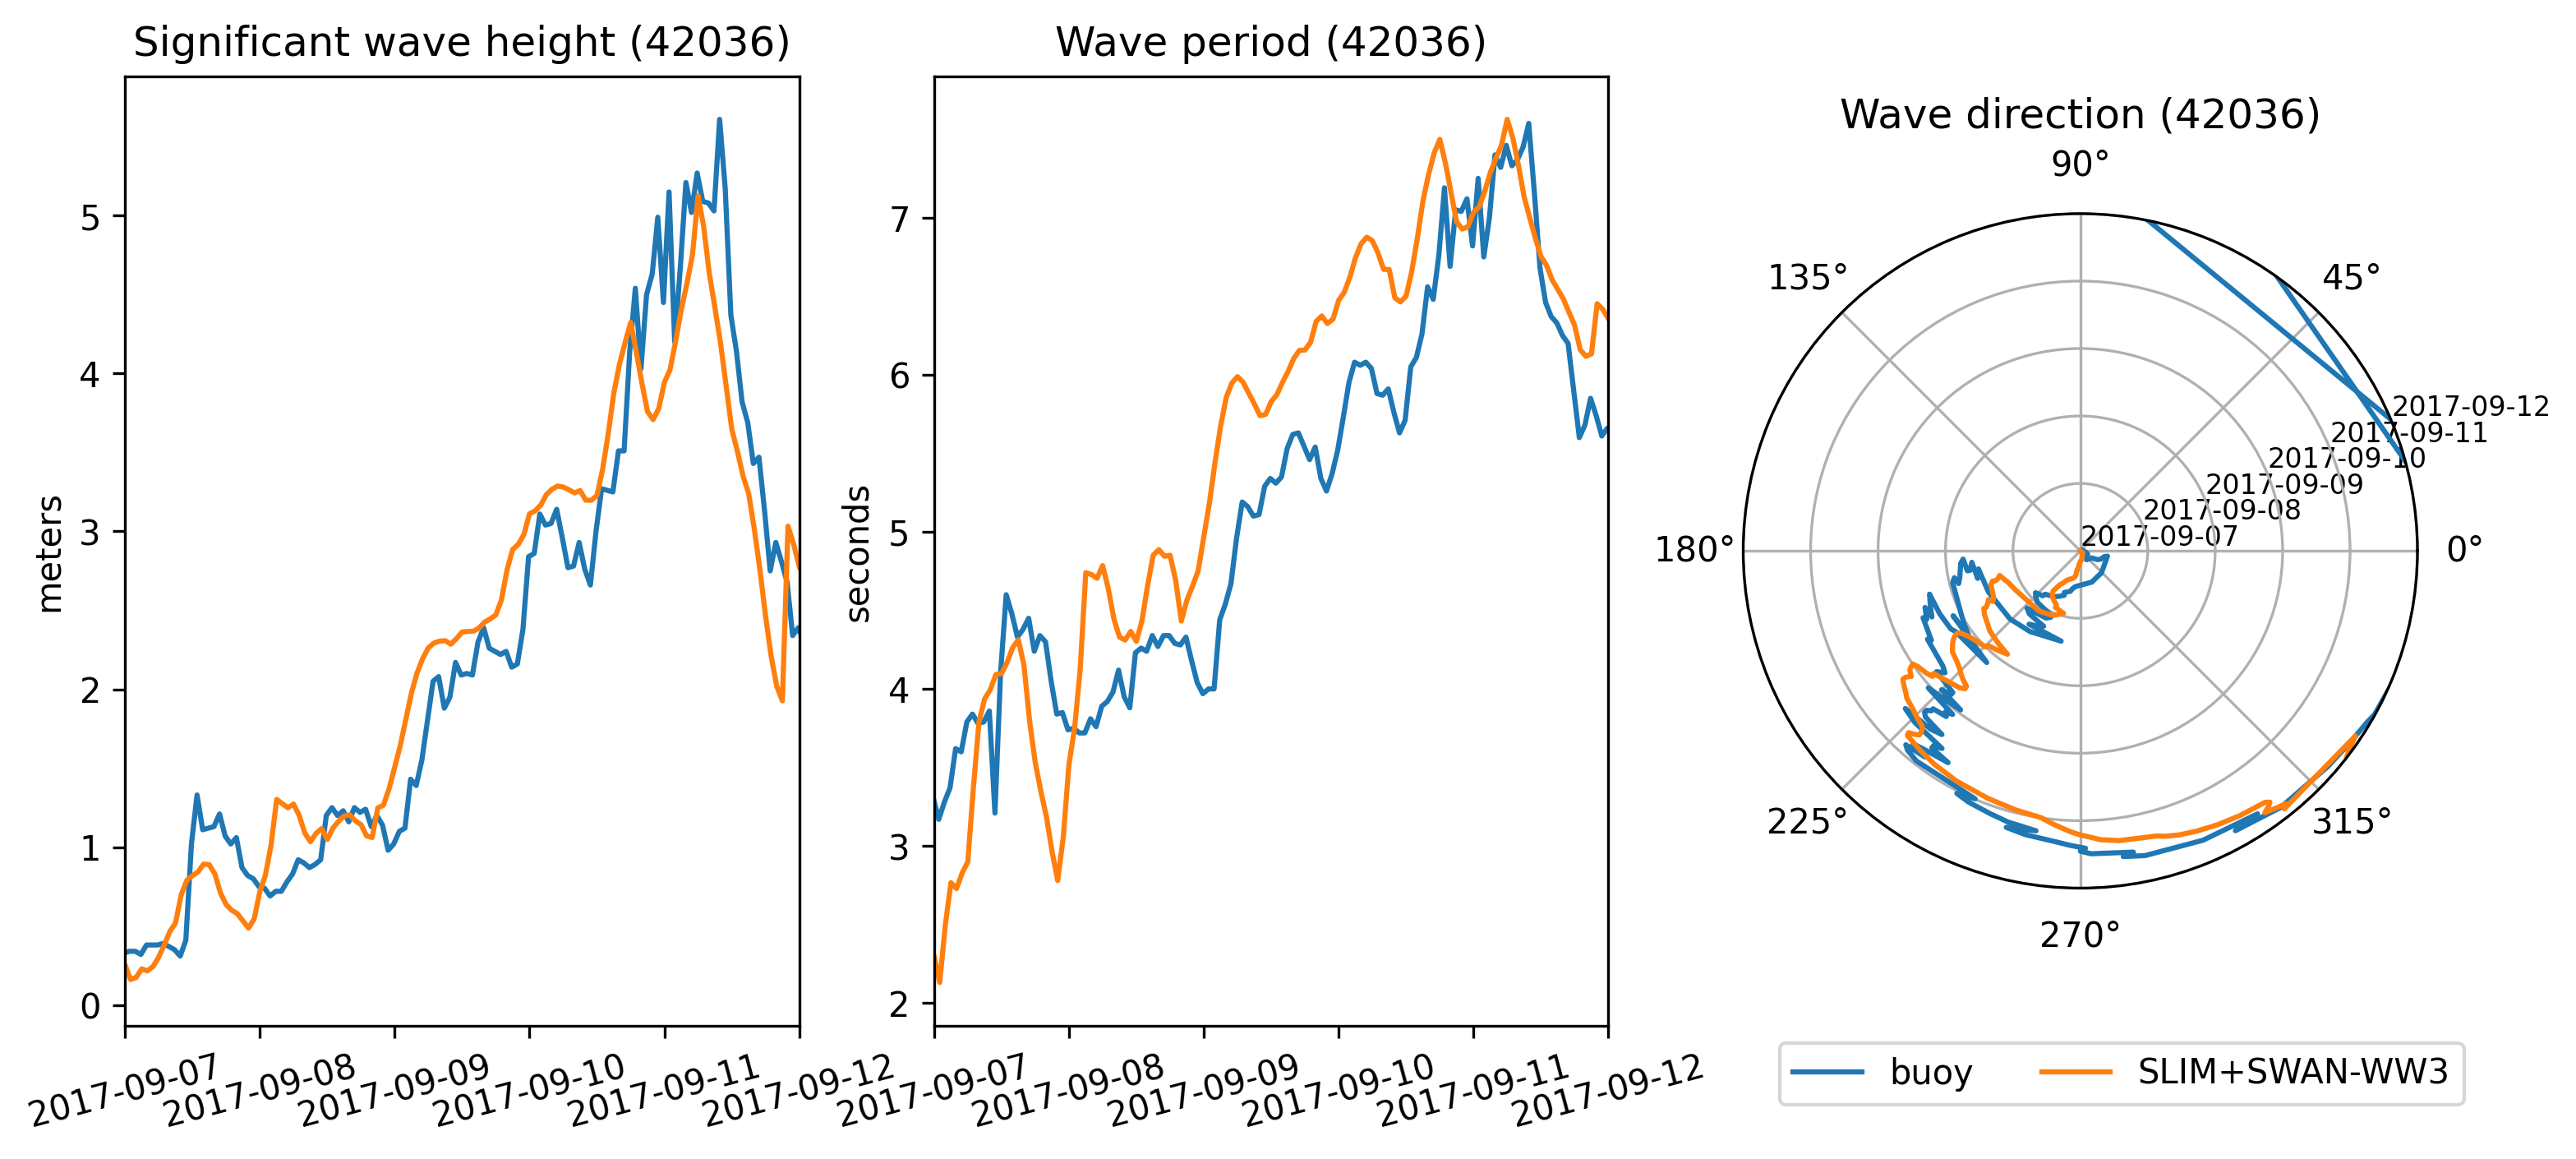
\includegraphics[width=.95\textwidth]{fig/val_waves.png}
    \caption{The significant wave height produced by the coupled model has been compared to buoy measurements at 4 different stations. The timing and amplitude of the peak during the hurricane is correctly reproduced for all stations. For station 42036, the period and direction of the waves also agree well with observations}
    \label{fig:waves}
\end{figure}

\subsection{Impact of waves}

\begin{figure}
    % TODO: Islands in Grey
    \centering
    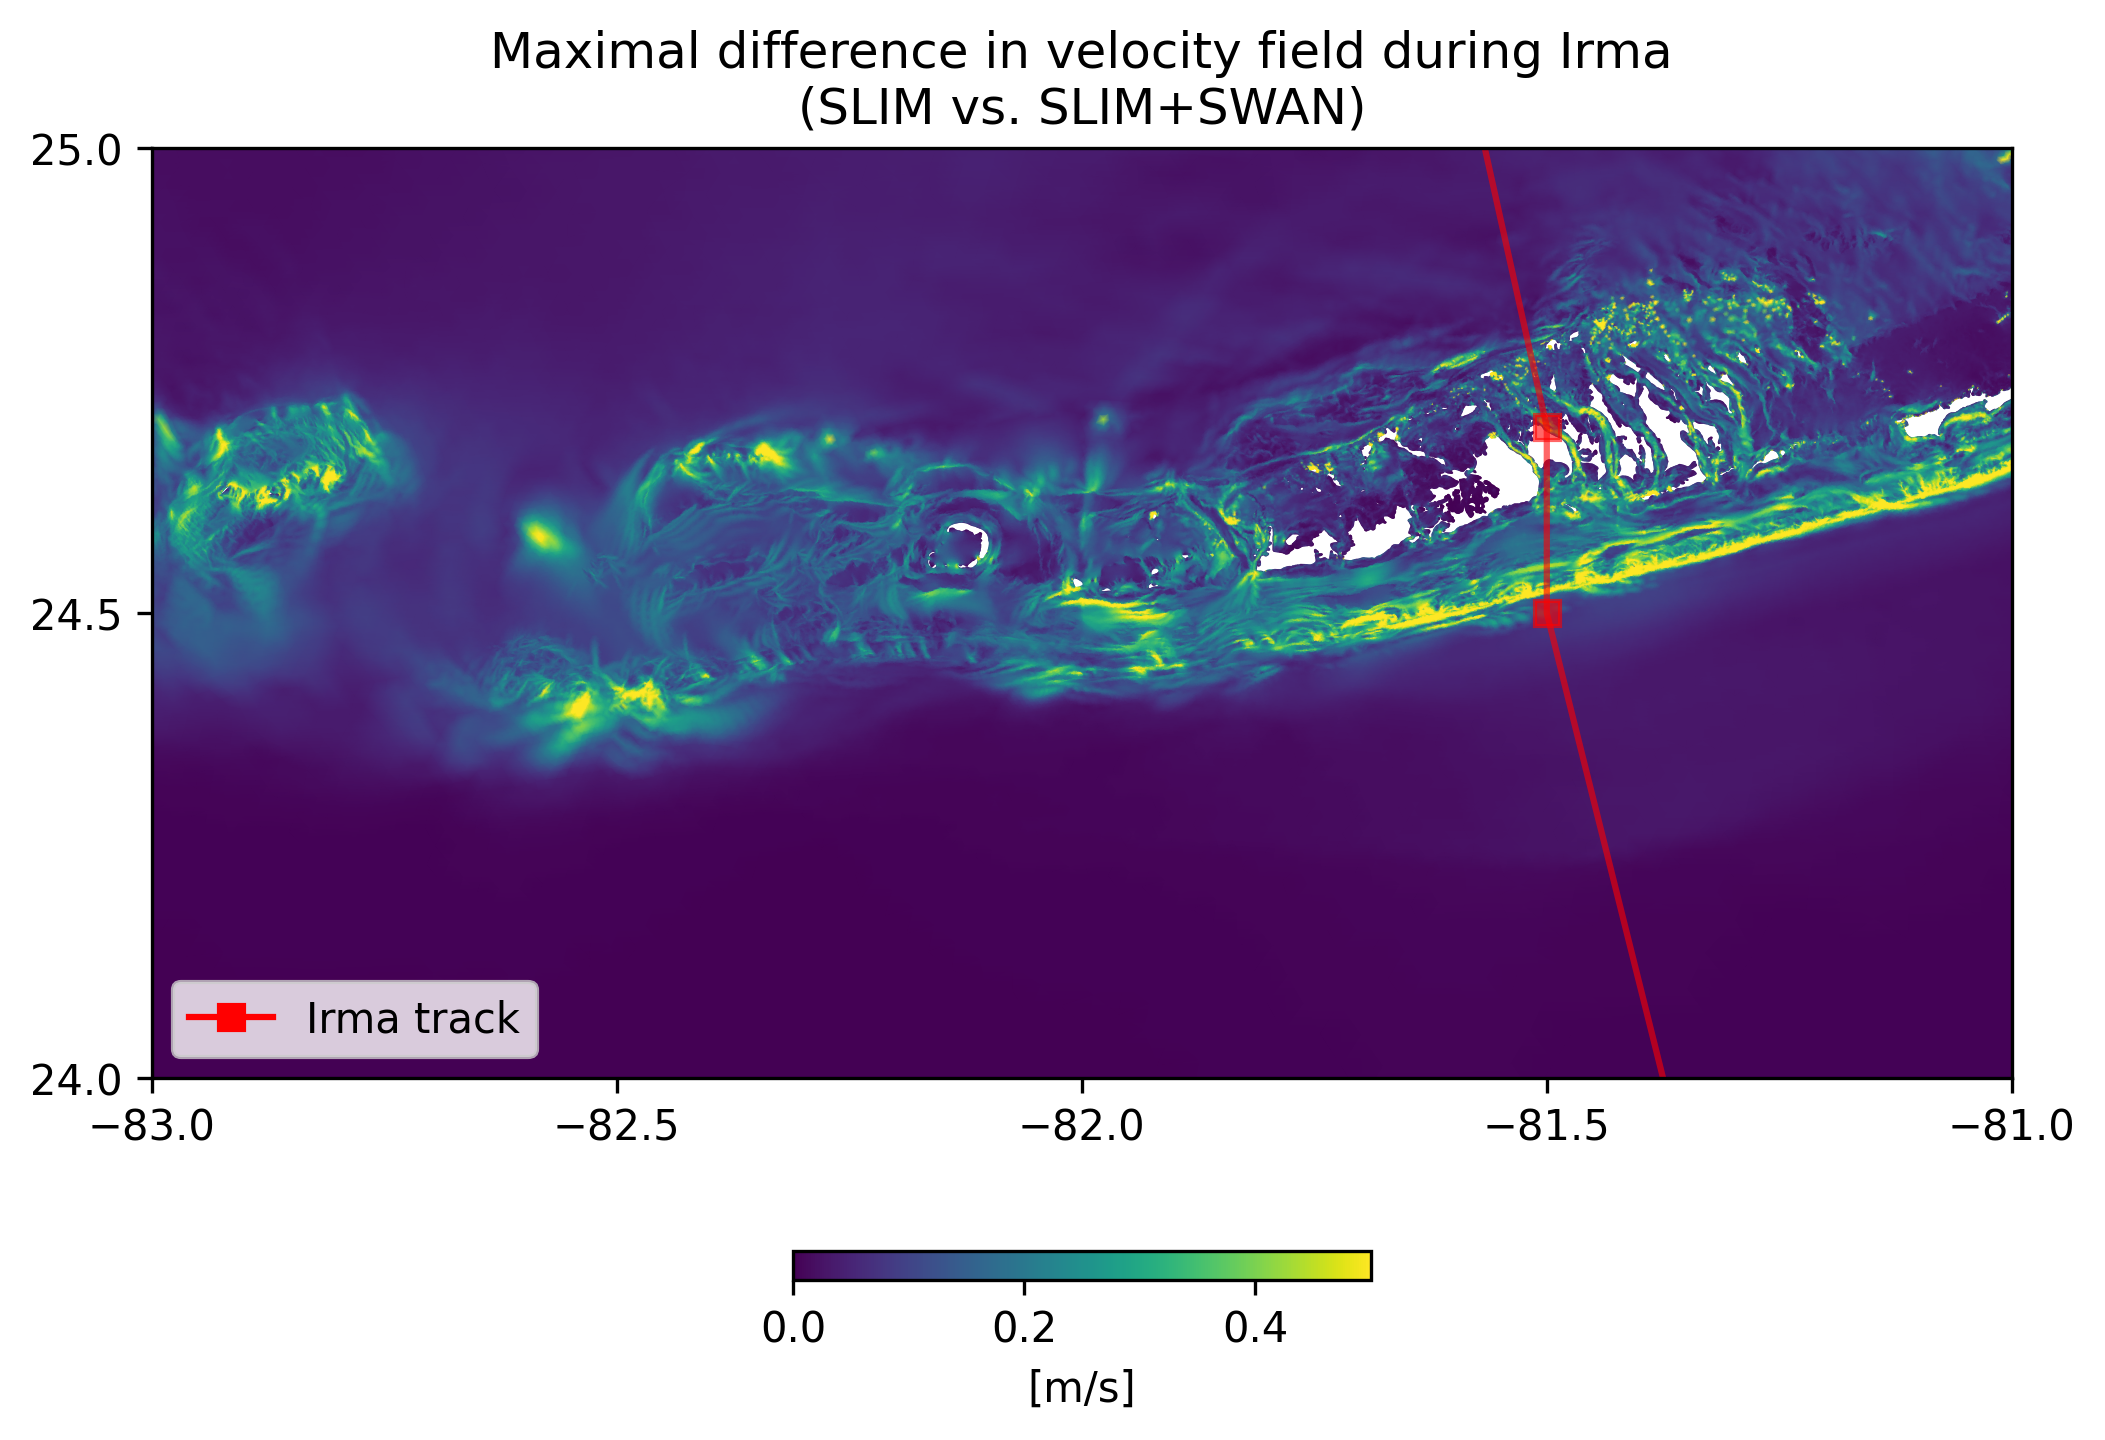
\includegraphics[width=.95\textwidth]{fig/max_diff_ww3.png}
    \caption{Maximum of the difference between SLIM and SLIM+SWAN currents speed between 2017-09-07 00:00:00 and 2017-09-13 00:00:00. The difference between the coupled and uncoupled model, which represents the effect of the wave-induced stress, can yield differences of 0.5 m/s in the simulated currents during the passage of the hurricane. SLIM+SWAN currents velocities are larger than the currents modeled by SLIM alone.}
    \label{fig:diff}
\end{figure}

\begin{figure}
    \centering
    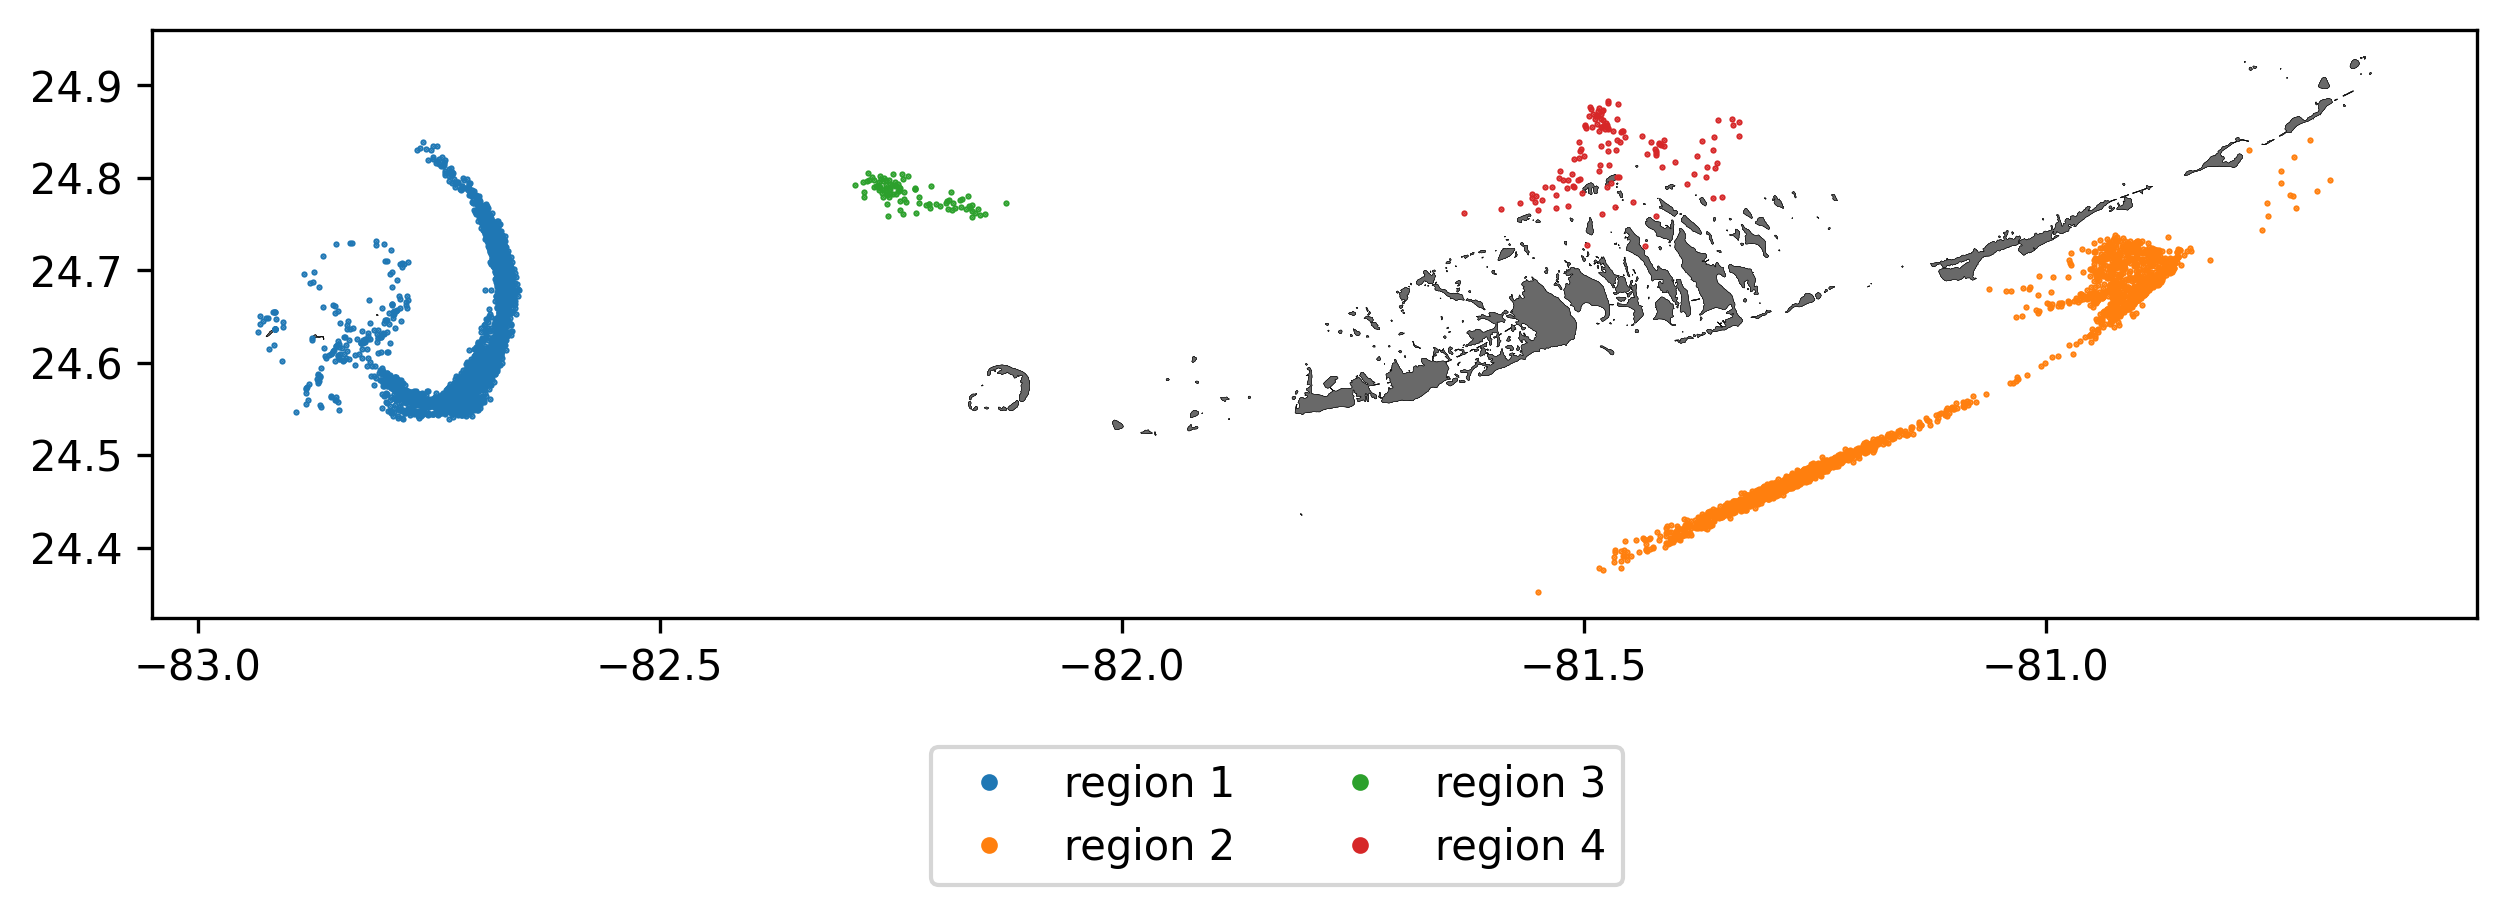
\includegraphics[width=.75\textwidth]{fig/release_regions.png}
    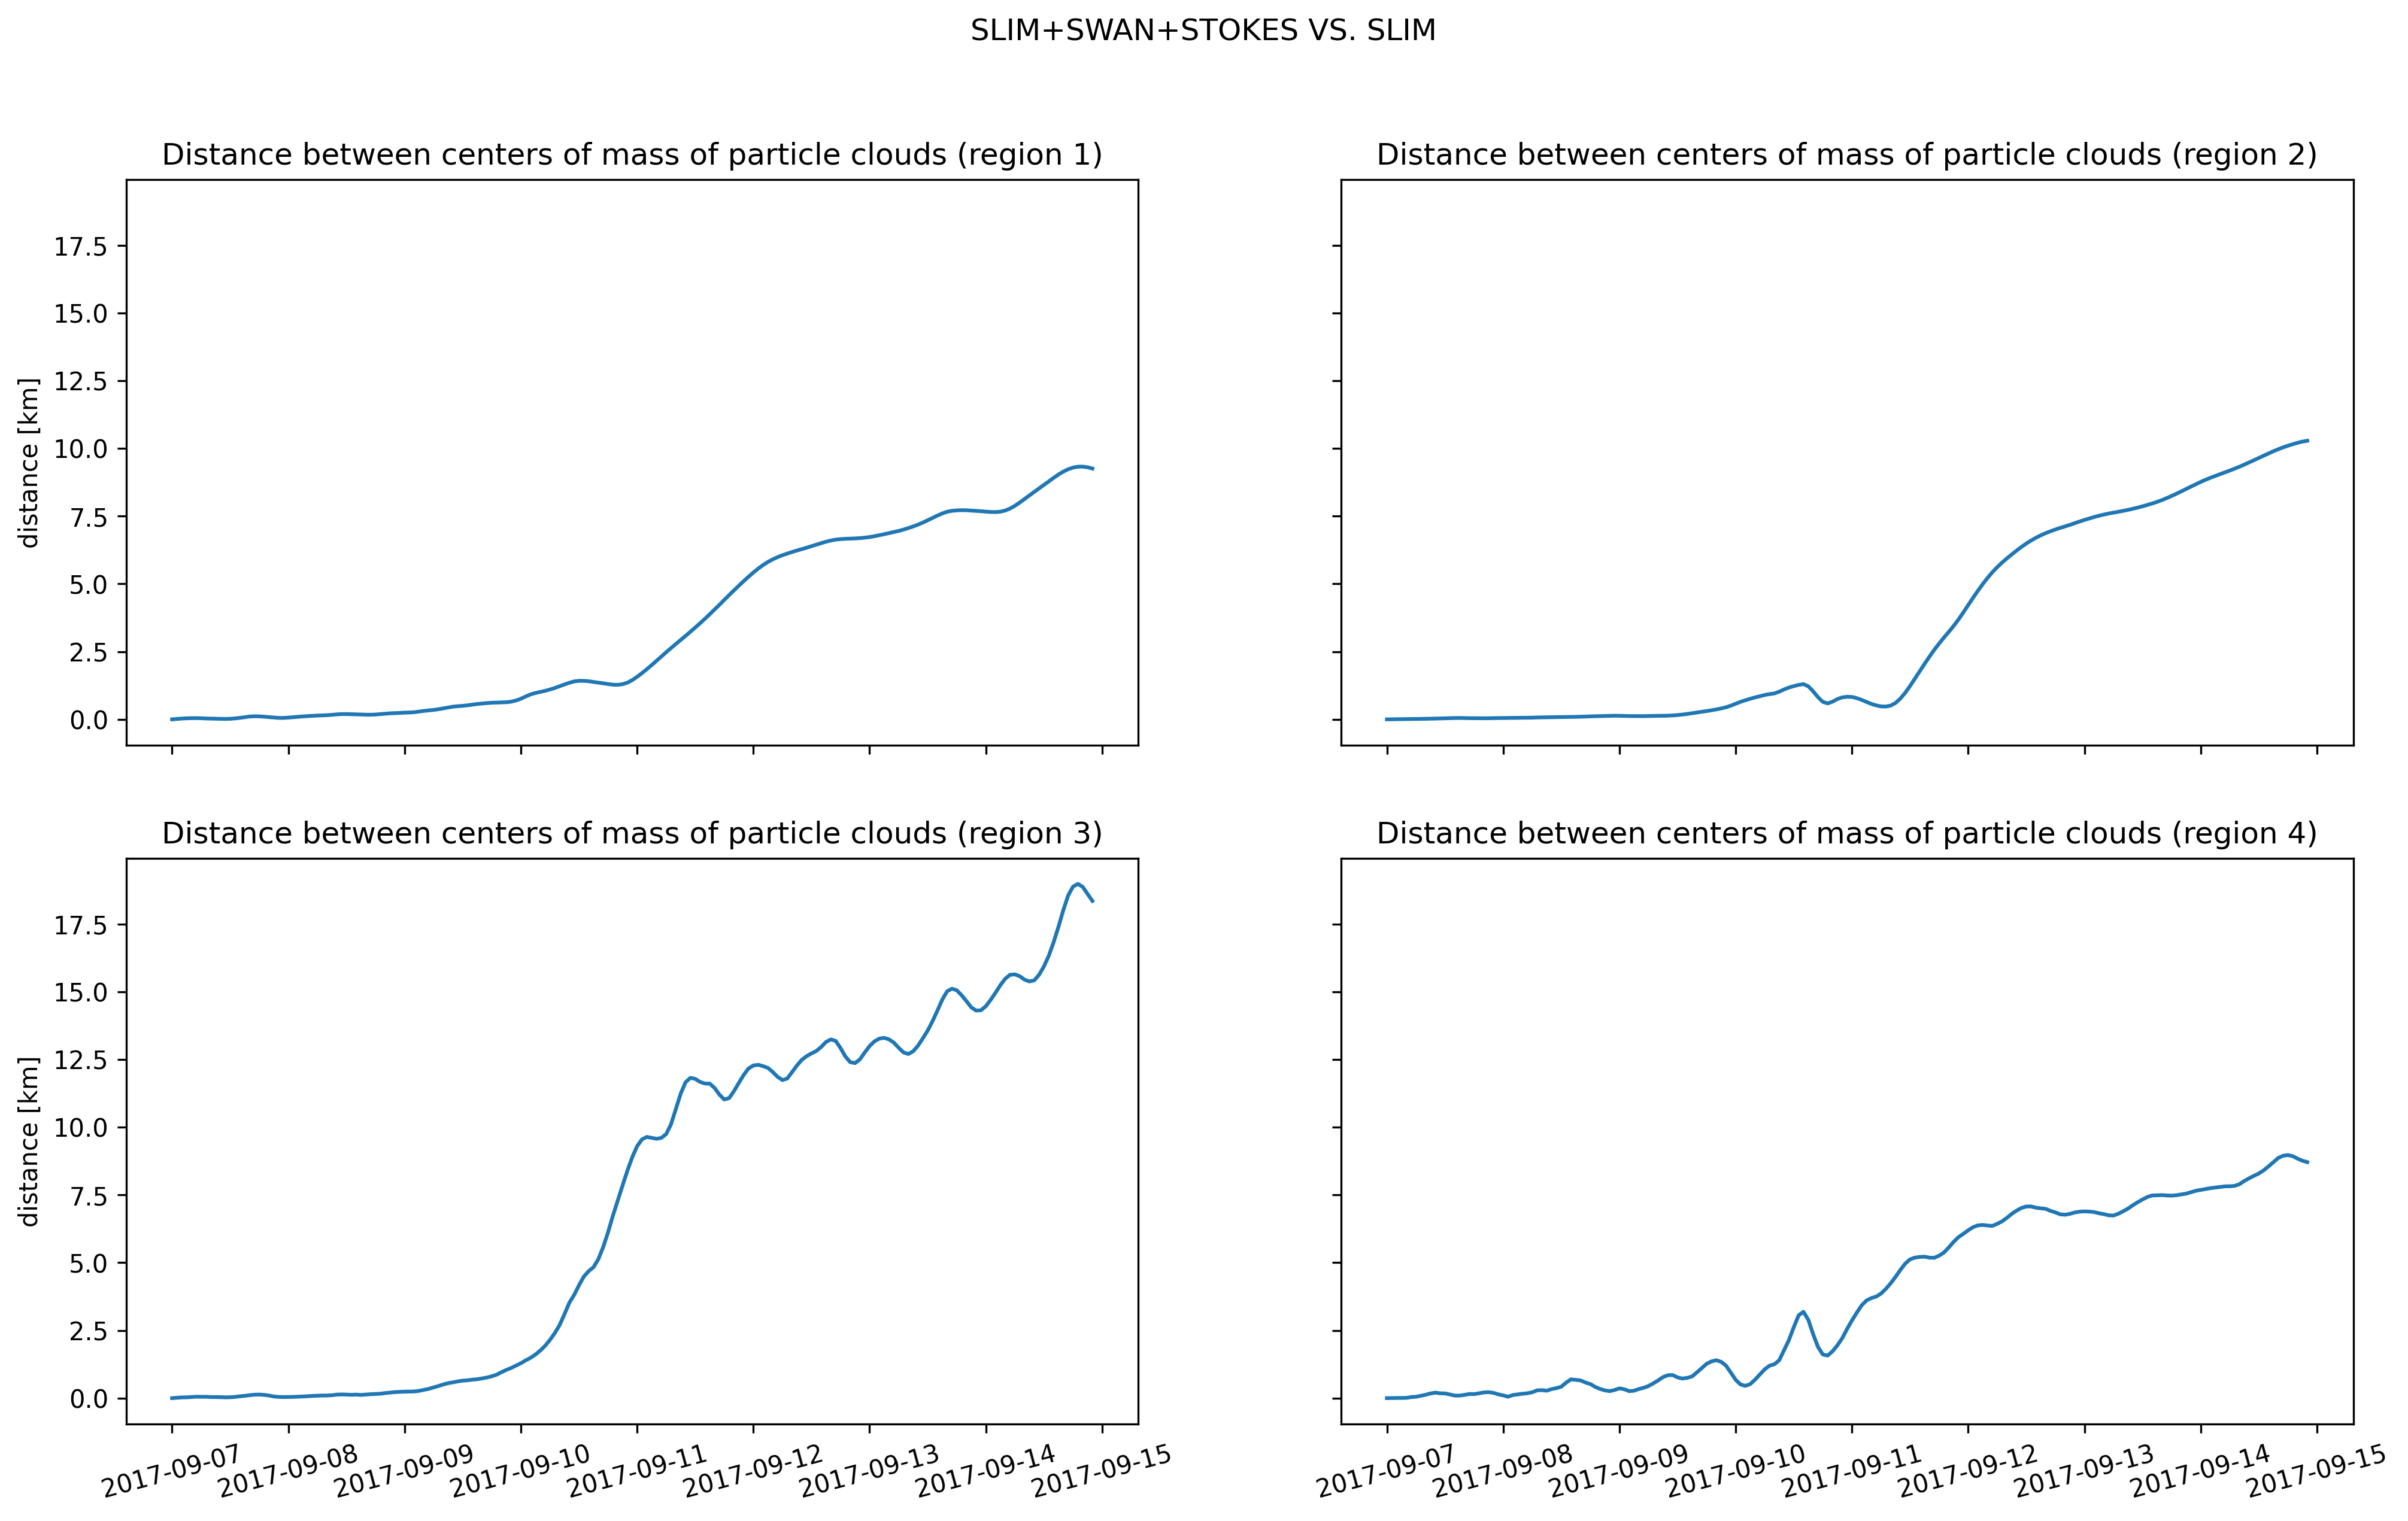
\includegraphics[width=.95\textwidth]{fig/slim+swan+stokes_vs_slim_WW3.png}
    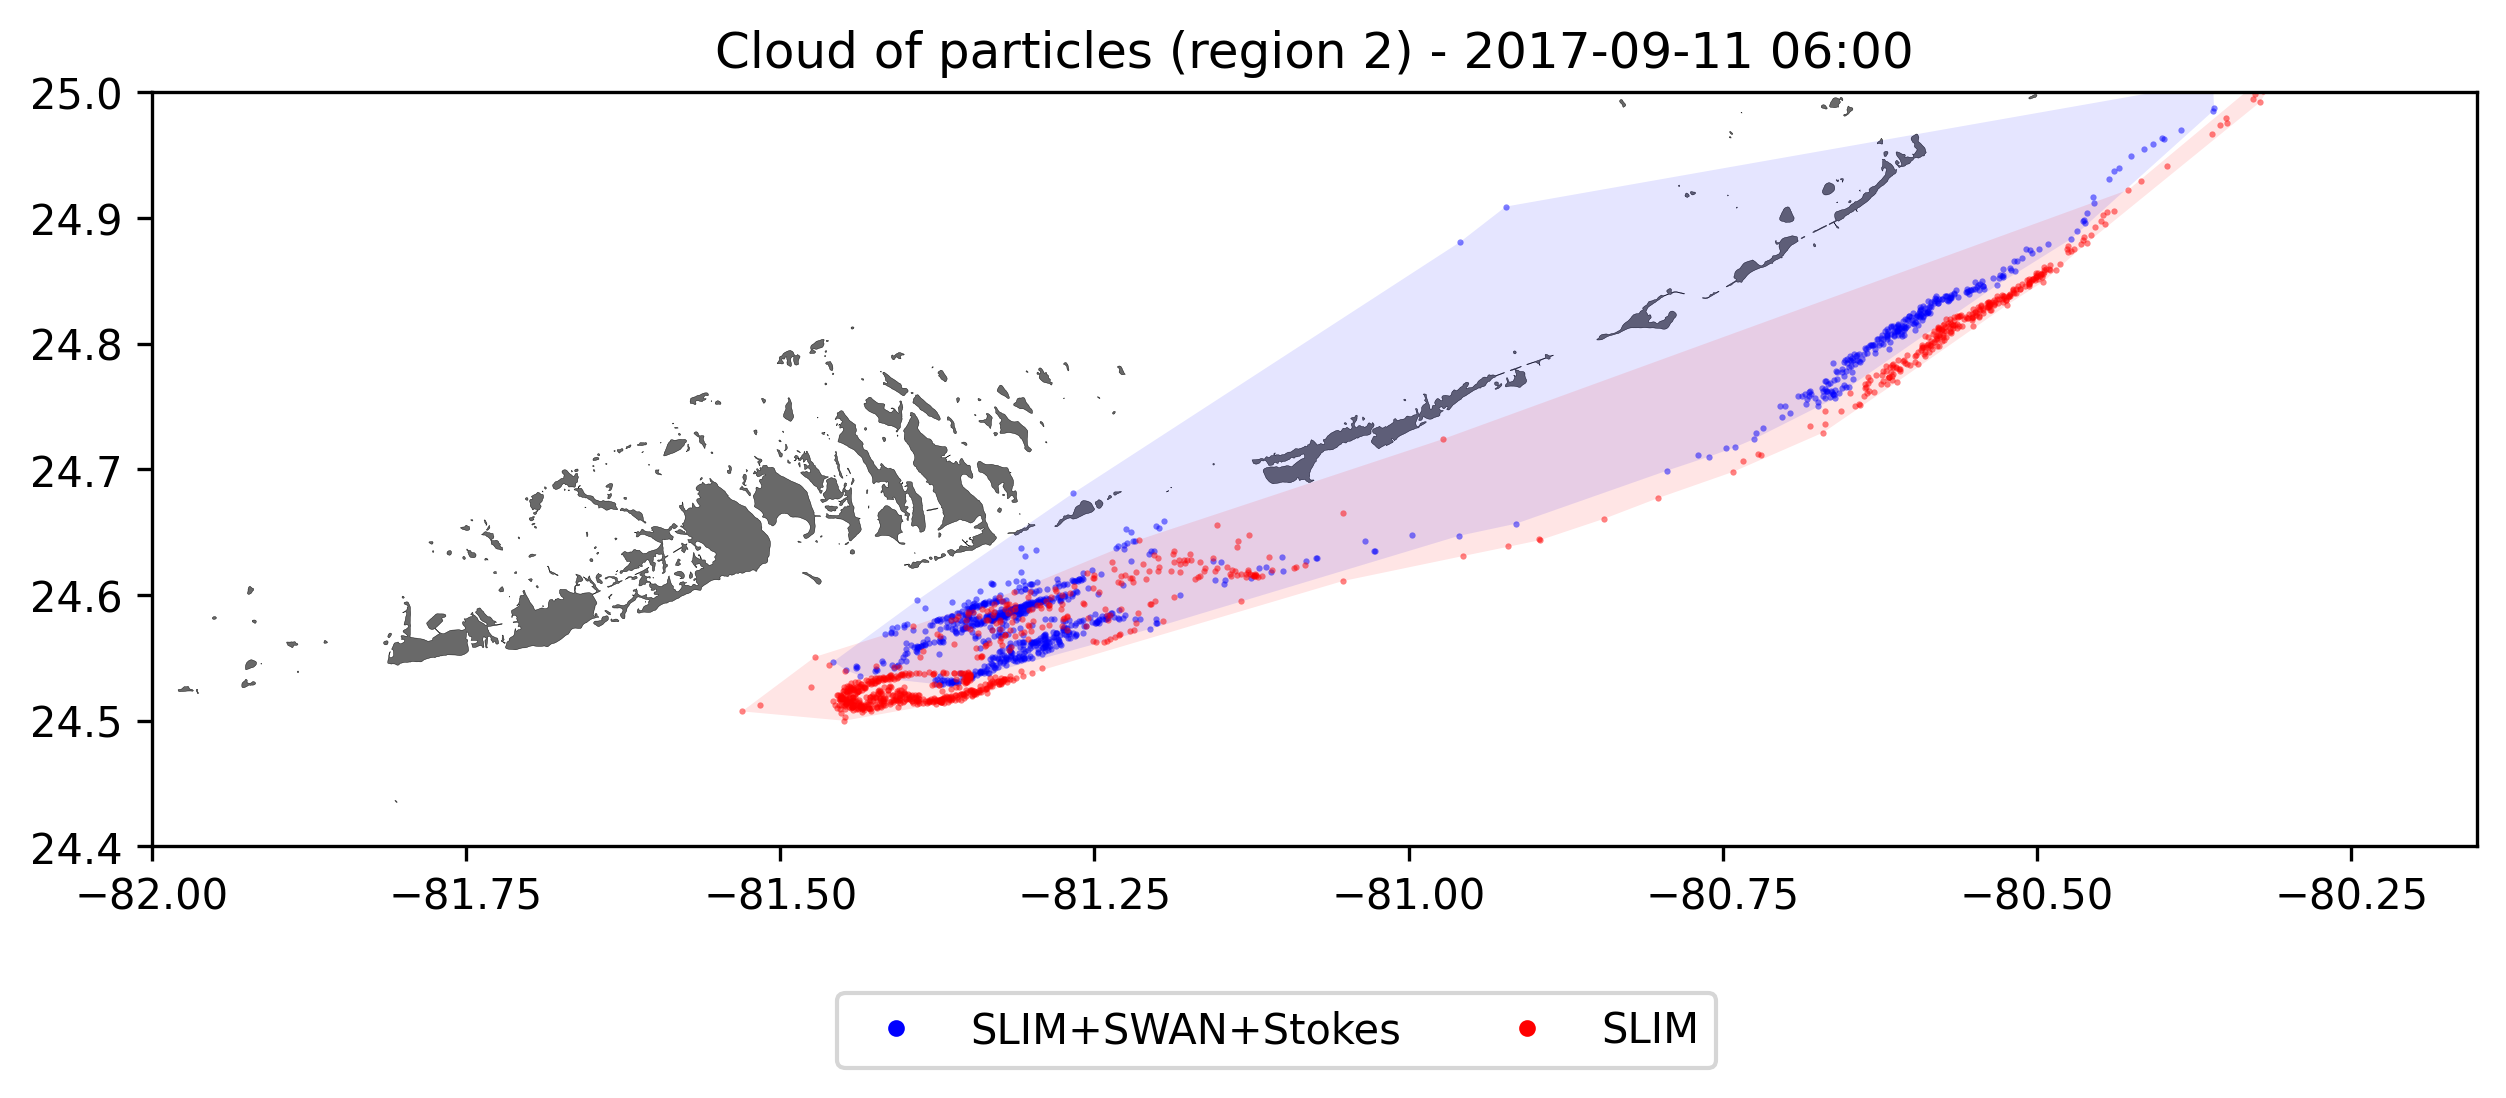
\includegraphics[width=.75\textwidth]{fig/matthieu_ww3.png}
    \caption{Comparison of passive drifters trajectories with SLIM+SWAN+Stokes drift vs. SLIM alone. A snapshot of the positions of the particles released from region 2 is shown after the passage of Irma in the Florida Keys. Particles advected by the currents of the coupled model tend to remain on the shelf while particles advected by SLIM alone are mostly transported along the shelf break}
    \label{fig:traj}
\end{figure}

% === DISCUSSION === %
\section{Discussion and conclusions}

Impact of waves on coral connectivity

Ability of wave model to correctly capture gradient in significant wave height due to current-waves interactions under tropical cyclones depends on:
\begin{itemize}
    \item Spatial (10km $\to$ 5km) and spectral (36 dir. $\to$ 48 dir.) resolution \citep{hegermiller2019wave}
    \item Directional spreading of incident waves \citep{villas2020wave}
\end{itemize}

\section*{Conflict of Interest Statement}
The authors declare that the research was conducted in the absence of any commercial or financial relationships that could be construed as a potential conflict of interest.

\section*{Author Contributions}
  
\section*{Funding}

\section*{Acknowledgments}
Computational resources were provided by the Consortium des \'Equipements de Calcul Intensif (\textsc{c\'eci}), funded by the \textsc{f.r.s.-fnrs} under Grant No. 2.5020.11. Thomas Dobbelaere is a PhD student supported by the Fund for Research training in Industry and Agriculture (\textsc{FRIA}/\textsc{FNRS}).

\section*{Supplementary Material}
The Supplementary Material for this article is attached to the submitted document.

% === BIBLIOGRAPHY === %
% \bibliographystyle{frontiersinSCNS_ENG_HUMS} 
\bibliographystyle{apalike}
\bibliography{./biblio.bib}

%%% Make sure to upload the bib file along with the tex file and PDF
%%% Please see the test.bib file for some examples of references

% \appendix
% \section*{Appendix}
% \renewcommand{\thesection}{A}
% \setcounter{figure}{0}
% \renewcommand{\thefigure}{\thesection\arabic{figure}}

\end{document}
